\chapter{Literature Review}
\label{litreview}
\lhead{Chapter 1. \emph{Literature Review}}

\section{Background}

An interesting definition of the Cloud Computing has
been written by the National Institute of Standards and Technology~\citep*{nistcloudcomputing}:

\begin{quote}
	“Cloud computing is a model for enabling ubiquitous, convenient, on-demand
	network access to a shared pool of configurable computing resources (e.g.,
	networks, servers, storage, applications, and services) that can be rapidly
	provisioned and released with minimal management effort or service provider
	interaction.”
\end{quote}

Different kind of clouds are specified, if Amazon is a “public” cloud, this is
not the only way to use a cloud infrastructure: private cloud or hybrid clouds
mixing private and public cloud infrastructures are being developed more and
more. Thanks to open-source projects like~\cite{websiteOpenstack},
cloud environments can be installed on private infrastructures. This is
sometimes necessary or requested for security, performance or data control
purposes.

The evolution of the paradigm of cloud computing has been made possible thanks
to different technologies. The virtualisation, as explained
by~\cite*{virtualisation} allows servers to be splitted in different
sub-components, isolated from each other, sharing the resources of the physical
machine. 

Technologies have been developed to give people much more flexibility in the
way to manage their virtual machines, also called instances. Actually, the
concept of live migration, which is detailed in the work
of~\cite*{livemigration}, has been built to move instances from one physical
host to another without interrupting the activity of anything running in the
virtual machine. The memory is kept intact of course, but also the running
connections.  The instance may seem frozen for a few second when the migration
is finalized, but nothing is disrupted.

\section{Motivation}

The legitimate question is “Why do people migrate their infrastructure to a
cloud infrastructure?”. The answers are multiple, Valentina Salapura explains
how a virtualized environment improves the resiliency of an
infrastructure~\citep*{virtresiliency}. More precisely, when a service requires
to be scalable, highly available and fault tolerant, using cloud technologies
is essential. In the case of disaster recovery scenarios, they are highly
simplified and cheaper thanks to those environments.

As a result the infrastructures are composed of a certain amount of physical
machines (PMs) which could be dispatched among different data centers, and each
of these PMs, contains a variable number of virtual machines (VMs). The
problematic which is now interesting concerns the assignment of these VMs, what
is the optimal distributions of the instances among the different servers? It
depends of what characteristic has to be optimized.

Thomas Setzer and Alexander Stage base their study on the statement that energy
represents up to 50\% of operating costs of an
infrastructure~\citep*{reassignmentElectricitysaving}. That's why there is a need
to optimize it. Using the virtual machine reassignment through live migrations,
they are looking at consolidating the VMs on the physical servers.
Consolidating an infrastructure consists in reducing the number of PMs which
are hosting instances without disturbing the performance of these.  After this
operation, useless PMs can be suspended and electricity is saved, then when
more computational power is required they are resumed dynamically.

In the publication \textit{An adaptive Resource Provisioning for the Cloud
Using Online Bin Packing}~\citep*{reassignmentBinpacking1}, the authors also
introduce their subject by explaining that it has been estimated that Amazon
manages more than half a million of physical servers around the world and that
it must be a priority for them to reduce their expenses by consolidating
their infrastructure.

\section{Algorithms}

We have seen that cloud computing is a hot topic in the Internet industry
which results in a lot of new problematics in computer science. The resource
allocation problem is one of them. All over the world, universities have
started studying different approaches of allocation optimisation. The different
algorithms listed in this document gather publications around the virtual machine
assignment and reassignment on a set of physical machines.

\subsection{Linear Programming}

Also known as Linear optimization. It is specialisation of mathematical
programming, which is focused on linear functions. The main goal of linear
programming is to find a maximum or a minimum to a linear function given a set
of constraints, in other words: maximizing profits while minimizing costs. In
scope of resource allocation, it is required to define the different variables,
the function we want to optimize and the constraints linked to the variables.

In their work,~\cite*{allocationHybrid} are working with linear programming. The aim
of their study is to define a way to optimize the number of allocated virtual
machines splitted in different cloud infrastructures.  Different constraints
are defined to setup the scope of the function to minimize.

\begin{figequation}
	\caption{Example of linear optimization problem}
	\[
		Minimize
		\sum_{k=1}^A \sum_{l=1}^{T_k} \sum_{i=1}^I \sum_{j=1}^C ( y_{klij} \cdot (ni_{kl} \cdot {pi_j} + no_{kl} \cdot po_j) + \sum_{s=1}^S ( p_{ij} \cdot x_{klijs} ))
	\]
\end{figequation}

\textit{Equation 1} is the problem they want to solve, in this case a cost
minimization problem. How can we minimize for each task $t$ of each application
$k$ in each virtual machine $i$ of each cloud infrastructure $j$ the price of
the input and output bandwidth ($ni \cdot pi_j$ and $no_{kl} \cdot po_j$) and
the price the requested virtual machines ($x_{klijs} \cdot p_{ij}$) at each
unit of time ($S$)

\begin{figequation}
	\caption{Example of constraints in a linear program}
	\[
		\forall j \in [1,C], s \in [1,S]:
		\sum_{k=1}^{A} \sum_{l=1}^{T_k} \sum_{i=1}^{I} cpu_i \cdot x_{klijs} \leq maxcpu_j
	\]
\end{figequation}

The \textit{Equation 2} defines a constraint from the linear problem, which
explains that in each cloud, at each unit of time, the sum of all the tasks run
on all the virtual machines instantiated should be less than the number of CPUs
available.  (There is note that in the case of public clouds, the amount of CPU
is considered unlimited so this constraint becomes void).

\vspace{1em}

The work of~\cite*{allocationHeterogeneous}, which
focuses virtual machine resources allocation in heterogeneous
environment also start by defining a formal
model based on linear programming. However, as explained in this publication,
resolving such a problem requires an exponential time, linked to the amount of
allocations to achieve. As a result using directly this solution on an
important workload is not feasible.

\vspace{1em}

The work of~\cite*{mathsRrndlp} about linear optimization
relaxation has been used to simplify the original problem
and transform it from an exponential complexity to a polynomial complexity. The
“random rounding” is a probabilistic approach which modifies some of the
constraints by a weaker one.

\begin{figequation}
	\caption{Application of random rounding}
	\[
		\text{constraint before: } 0 \leq x \leq 1 \\
	\]
	\[
		\text{constraint after: } x_r \in {0, 1}
	\]
	\[
		x_r = 1 \text{ with a probability of $x$, otherwise: $0$}
	\]
\end{figequation}

However, the RRND approaches is quickly discarded as the results are not good
enough in the case of resource allocations in heterogeneous environment.

\subsection{Bin packing}

Bin packing is one of the most common approach to resource allocation or
re-allocation in a cloud environment. It consists in representing “bins”
associated to a storage capacity and “items” which have to be packed into
those bins.

\subsubsection{Different variants}

Two main types of bin packing algorithms exist. On the one hand, those
considered as “offline”. They consider that we have access to all the items to
find the optimal packing on the different bins. This problem is a NP-hard
problem, there is no, to this day, a polynomial way to solve this problem.
That is why to answer this problem in a reasonable duration, different
heuristics have to be defined. The most common have been studied
by~\cite*{mathsBpheuristics}:

\vspace{1em}
\begin{center}
	\begin{tabular}{| l | p{7cm} |}
		\hline
		Algorithm Name & Description \\
		\hline
		First Fit (FF) & Pack the item in the first bin with a large enough capacity \\
		\hline
		Best Fit & Pack the item in the bin which will have the less capacity after packing \\
		\hline
		Worst Fit & Opposite of Best Fit: Pack the item in the bin with the biggest capacity \\
		\hline
		Next Fit & Same as FF except that instead of reconsidering the first bin after packing, the current one then the next one is considered \\
		\hline
		*-Fit Decreasing & First, sort the items in a decreasing order, then apply any of the *-Fit algorithm \\
		\hline
	\end{tabular}
\end{center}
\vspace{1em}

Those different algorithms reduce the complexity of the packing operation to
$O(n\log{n})$. But as~\cite{mathsBpheuristics} title explains: they are
“Near-Optimal”. The issue is finally to find the best ratio optimality/complexity.

On the other hand, the “online” algorithms, which, on the contrary, are packing
items at the time they are arriving. In this case bins are already partially
filled with other items, and it is not always possible to move those. Thus, the
main goal is to find the best assignment for the newly coming item. Previous
*-Fit could be directly used. However, it is really limited to pack one item in
a set of bin, this is why different algorithms have been developed

To answer more precisely to the cloud resource allocation problem, some people
have defined some variants of those two main categories of bin packing
algorithms. G. Gambosi and A. Postiglione and M. Talamo have developed a
“relaxed online bin packing” algorithm~\cite*{mathsRelaxedonlinebp}. It may be
represent as a mix between online and offline bin packing. When a new item has
to be packed, it allows an additional limited number of moves among the
currently packed items.

Another interesting variant is the dynamic online bin packing defined by Joseph
Wun-Tan.  It differentiates itself from standard online bin packing by allowing
items to be removed from bins. Static online bin packing does not allow these
items changes, once an item has been placed it does not move anymore.

\subsubsection{Their application in resource allocation}

In the scope of virtual machines assignment on physical hosts, the bins are the
physical servers and the items are the virtual machines we want to assign,
and consequently, the services or tasks we want to host. Some additional aspects
have to be considered: virtual machines need different resources like memory,
CPU, persistent storage (disk), network input/output. So often, the items we
want to pack are multidimensional items, and we speak of multidimensional
vector bin packing. Another interesting point is that moving a virtual machine
from one host to another has a cost which may be important, and which prevent 
doing numerous migrations in the meantime.

In the work about online bin packing for virtual machines allocation
of~\cite*{reassignmentVisbp}, the authors consider first, that a virtual
machine only has one dimension, its CPU consumption. From that point they study
which algorithm may fit this particular problem. They reject “strict” online
bin packing, because in realistic situations it is uncommon to know exactly
the future consumption of a virtual machine, so it is necessary to move it
afterward, when we can measure it. Moreover, as VMs can be migrated easily,
there is no reason not considering it if the resulting performance is better.
“Relaxed online bin packing” allows movements when a new item is packed, but
an item cannot be resized. “Dynamic online bin packing” is thought inadequate
in this context too, but often, when an virtual machine has to move the best
solution is not always to remove it then repack it, but to move others instances
which are easier to move.

This is why in\cite{reassignmentVisbp}, they decided to build an online bin
packing algorithm which suits the virtualisation environment: “Variable Item
Size Bin Packing”, its characteristics are the following.

\begin{itemize}
	\item{As relaxed online bin packing, it allows movements when a new item is packed}
	\item{Stronger limit of movements, to avoid executing too many migrations}
	\item{A \texttt{change} operation is defined to modify the size of an item in a bin}
\end{itemize}

They extend their algorithm to multidimensional vectors by considering the biggest
value among the different dimensions of a vector, so the problem returns to
one-dimension. Using this way to simplify the problem is working in some cases.
Commonly when a resource consumption increases the others are following. For
example an application having a high network bandwidth requirement, would also have a
high CPU consumption. Finally, they admit that this solution would work quite poorly
in the case of instances with non-proportional requirements.

In~\cite{allocationHeterogeneous}, we have seen that the first approach of the author
was around linear programming, but the main part of their work is defining a way
to apply multidimensional vector bin packing to heterogeneous environments. On a first side,
they deal with the multidimensional aspect of this problem. It is necessary to specify how to
sort the items because there is not natural way to sort these vector.

\begin{itemize}
	\item Value of the maximal dimension
	\item Sum of all dimensions
	\item Ratio of the max/min
	\item Difference max-min
	\item Lexicographic order
	\item None
\end{itemize}

Most of the previous algorithms are not considering the way the bins are used.
In this publication, as it is targeting heterogeneous infrastructure, the order
the bins are sorted when executing any algorithm matters. All the previous way to
sort the items can be applied to the set of bins.

All these previous possibilities of ordering among the virtual machines and physical
hosts are combined and result in a “meta” algorithm (METAHVP) which takes the best result
out of the different combinations of one items ordering and one bins ordering. After
individual analysis, some sort types are removed from the meta algorithm to improve
its runtime. (METAHVPLIGHT)

The simulation achieved to test these heuristics are comparing the results to those
which have been found using the linear programming method and those obtained using
greedy algorithms (*-Fit). The conclusion is that METAHVP has the best results over
all the other, and METAHVPLIGHT achieves this result in on tenth of METAHVP's runtime.

Finally, according to what we want to study there are several possible solutions using
bin packing. Semantically, it is really comfortable to compare bins with physical servers
and items with virtual machines, it allows a very natural vision of this problem.

\subsection{Others}

To deal with mathematical optimization and approximative solution of NP-complete problems,
Ants colony algorithms, genetic algorithms and some other famous methods, based on statistical
analysis.

\subsubsection{Ant colony algorithms}

In~\cite{algoAntcolony1},~\cite{algoAntcolony2} and~\cite{algoAntcolony3}, the ant colony
algorithms are studied. As we can see in the following graph:

\begin{figure}[H]
\begin{center}
	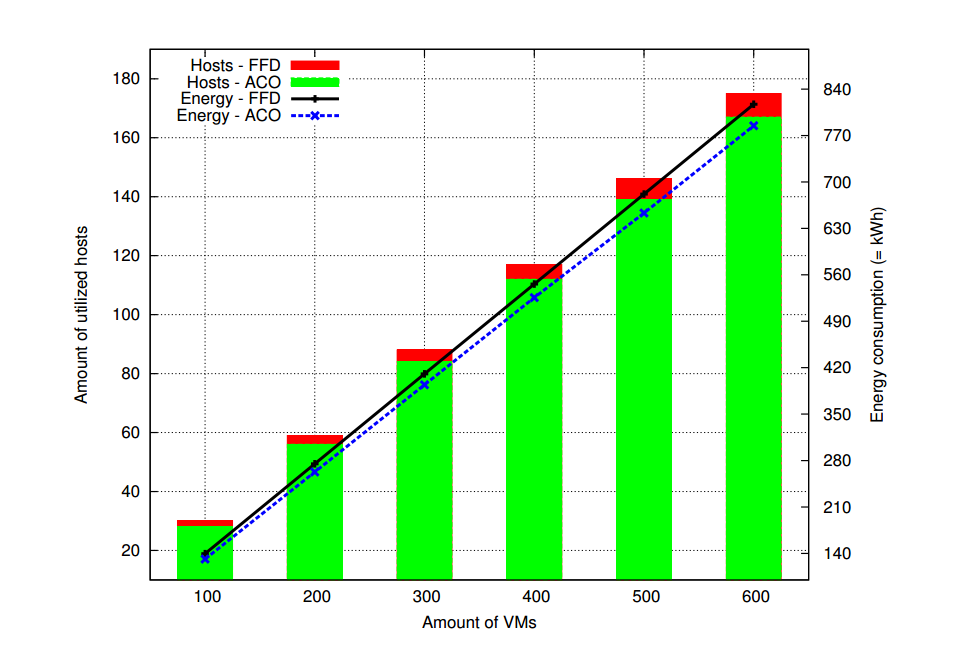
\includegraphics[width=0.8\textwidth]{./Images/antcolonyperf.png}
	\caption{Comparison between First Fit Decreased and Ant Colony algorithms in~\cite{algoAntcolony2}}
\end{center}
\end{figure}

The simulation shows that the ant colony gets better performance than a simple greedy First
Fit Decreasing, however this improvement is not free:

\begin{figure}[H]
\begin{center}
	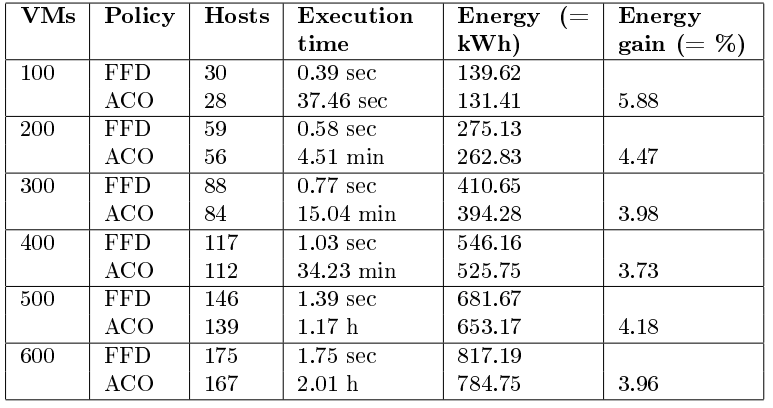
\includegraphics[width=0.6\textwidth]{./Images/antcolonyruntime.png}
	\caption{Runtime of First Fit Decreased and Ant Colony algorithms in~\cite{algoAntcolony2}}
\end{center}
\end{figure}

When the number of nodes becomes bigger, the time spent to find the optimal
allocation grows hugely, it is thousands times longer than a simple First Fit
Decreasing for 3 to 5 percents of improvement. For analysis purpose it is
something interesting to get better results, but in a realistic point of view,
this operation can not take several hours as it should be repeated often.

\subsubsection{Genetic algorithms}

Genetic algorithms (GA) are heuristics based on natural selection. Generations
of solutions are mutating, inheriting with and from each other to result in
close to optimal results.~\cite{algoGenetics1} and~\cite{algoGenetics2}
focused on them to solve the virtual machines assignment problem. In the work
of David Wilcox et al.\cite{algoGenetics1}, simulations are comparing GA with
*-Fit algorithms.

\begin{figure}[b!]
\begin{center}
	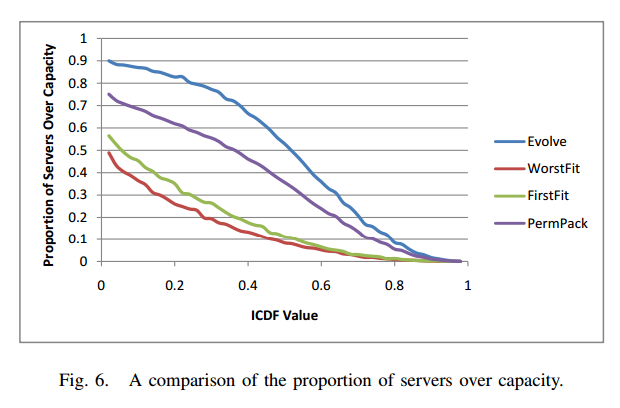
\includegraphics[width=0.65\textwidth]{./Images/geneticperf1.png}
	\caption{Results of simulations using a genetic algorithm\cite{algoGenetics1}}
\end{center}
\end{figure}

\begin{figure}[H]
\begin{center}
	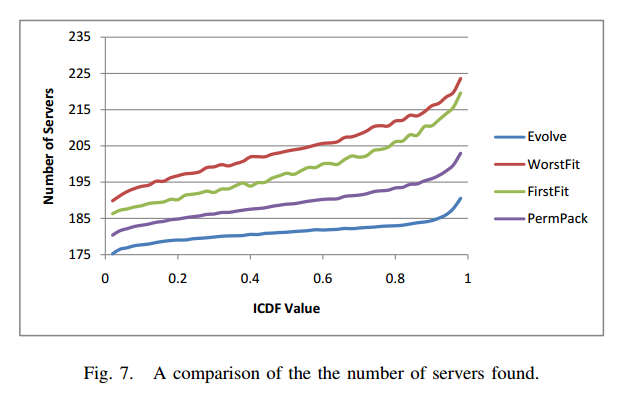
\includegraphics[width=0.65\textwidth]{./Images/geneticperf2.png}
	\caption{Results of simulations using a genetic algorithm\cite{algoGenetics1}}
\end{center}
\end{figure}

On the following graphs, ICDF stands for “inverse cumulative distribution
function” also known as “quantile function”, the authors use it to represent
the load: “Using the icdf, we can specify a percentile value and obtain a
corresponding load which can be passed to the assignment algorithm”.

The conclusion which is that GA tends to consume less physical hosts, at any
load, the number of PMs is largely under the amount of servers used by the
other bin packing algorithms. As a direct consequence, the PMs which are
over-capacitated (where the amount of VMs exceed the resource capacity of the
physical sever), is much more high. For this reason, this approach can hardly
be used in environment where a SLA (Service Level Agreement) has to be
respected, because if there are overloaded servers, some applications or tasks
running of them will be slowed by this situation.

\subsubsection{Network flows}

Network flows are basically directed graphs where each edge has a capacity and a flow.
The main property is that each node of this graph must have an equal sum of flows from
the edges directed to it and leaving from it, except for two particular type of nodes:
“the source node” and “the sink node”.

\begin{figure}[H]
\begin{center}
	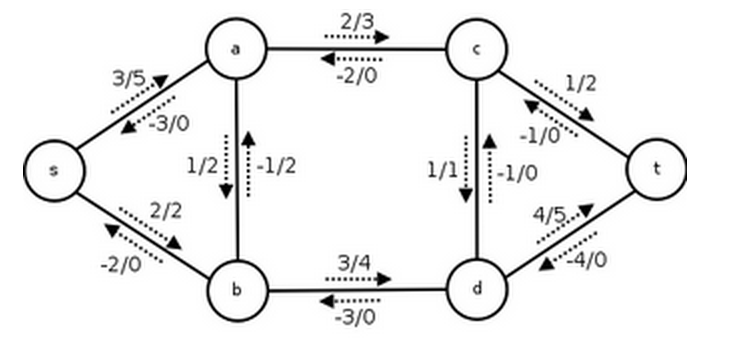
\includegraphics[width=0.8\textwidth]{./Images/examplenetwork.png}
	\caption{Example of network flow directed graph}
\end{center}
\end{figure}

Some people have used this concept to build a model to solve the resource
allocation problem, to fine a close to optimal solution. Kimish Patel, Murali
Annavaram and Massoud Pedram worked on resource assignment in
datacenter\cite{allocationNetworkflow}, considering an heterogeneous
environment as in~\cite{allocationHeterogeneous}. Each set of similar servers,
considered as a pool of servers is represented by a node, with a capacity
different from each other according to the differences between two pools of
servers.

Unfortunately, this technique does not seem to be used for virtual machines
allocation, and the link between this method and the problem we are dealing
with is not obvious at all.

\section{Real data analysis}

Most of the cited works in the literature review are basing their work on
simulations.  In the experiments, simulation tools like
SimGrid\cite{websiteSimgrid} or CloudSim\cite{websiteCloudsim} are used to simulate
the behavior of one or multiple cloud infrastructures.

The data may be generated randomly or following some statistical rules, but
often, workloads are based of extract of real workload. Typically, Google is
releasing workloads of its own production infrastructure. 

In 2012, Google sponsored the ROADEF contest (Operational research and decision
support French society)\cite{websiteRoadef}. The contest was focusing the machine
reassignment problem based on Google workload. Each attendee had to find the
best solution find solution. Some of them resulted in an official publication
like “Heuristics and matheuristics for a real-life machine reassignment
problem” from Ramon Lopes, Vinicius W.C. Morais, Thiago F. Noronha and Vitor
A.A. Souza\cite{roadefIp}.  They based their work on linear programming.
However in~\cite{roadefBp1} and~\cite{roadefBp2}, the authors have used
around the bin packing algorithms. Unfortunately, the work of the winner has
not been published so we are not able to see which algorithm has been used to
achieve the best reassignment.
